\documentclass{article} % For LaTeX2e
\usepackage{nips15submit_e,times}
\usepackage{hyperref}
\usepackage{url}
%\documentstyle[nips14submit_09,times,art10]{article} % For LaTeX 2.09
\usepackage{caption}
\usepackage{listings}
\usepackage{graphicx}
\title{Weekly Report(July.22.2019-July.28.2019)}


% The \author macro works with any number of authors. There are two commands
% used to separate the names and addresses of multiple authors: \And and \AND.
%
% Using \And between authors leaves it to \LaTeX{} to determine where to break
% the lines. Using \AND forces a linebreak at that point. So, if \LaTeX{}
% puts 3 of 4 authors names on the first line, and the last on the second
% line, try using \AND instead of \And before the third author name.

\newcommand{\fix}{\marginpar{FIX}}
\newcommand{\new}{\marginpar{NEW}}

%\nipsfinalcopy % Uncomment for camera-ready version

\begin{document}


\maketitle

\begin{abstract}
This week I continue to train Resnets and get an average accuracy of 95\%. And this mini project seems to come to an end.

\end{abstract}

\section{Question from last week}

\begin{itemize}
\item First, I run more different models to ensure it is not a coincidence. The result are shown at Table 1. The performances are relatively steady and still worse than SGD's. Therefore, the phenomenon I metioned last report still exists. It seems not a coincidence. 

\begin{table}[h]
\caption{momentum=0.95, epochs=100}
%\label{sample-table}
\begin{center}
\begin{tabular}{c|c|c}
\multicolumn{1}{c}{\bf Learning Rate} & \multicolumn{1}{c}{\bf Batch Size} &\multicolumn{1}{c}{\bf Accuracy}
\\ \hline \\
0.01 & 256 & 78.42\% \\
0.003 & 256 & 74.21\% \\
0.001 & 256 & 72.33\% \\
0.0003 & 256 & 63.17\% \\
0.0001 & 256 & 47.81\%
\end{tabular}
\end{center}
\end{table}

\item The loss curves are shown in Figure 1. obviously when learning rate becomes smaller, model need more epochs to converge. Last report I didn't realize this since models optimized by SGD can all converge in 100 epochs. Sorry about this mistake.

\item Give the model larger learning rate and it can indeed converge in 100 epochs with a good performance. The results are shown in Table 2 and loss curves are shown in Figure 2.

\begin{table}[h]
\caption{momentum=0.95, epochs=100}
%\label{sample-table}
\begin{center}
\begin{tabular}{c|c|c}
\multicolumn{1}{c}{\bf Learning Rate} & \multicolumn{1}{c}{\bf Batch Size} &\multicolumn{1}{c}{\bf Accuracy}
\\ \hline \\
1 & 256 & 87.29\% \\      
0.3 & 256 & 87.97\% \\
0.1 & 256 & 86.58\% \\
0.03 & 256 & 83.41\% \\
\end{tabular}
\end{center}
\end{table}

\begin{figure}[htbp]
\centering
{
\begin{minipage}[t]{0.45\textwidth}
\centering
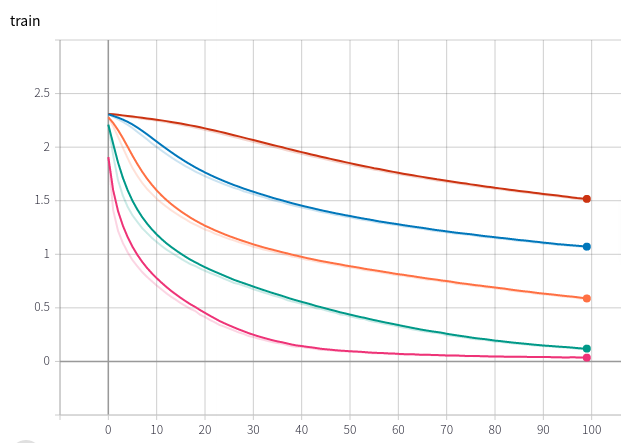
\includegraphics[scale=0.4]{1.png}
\caption{small learning rate}
\end{minipage}
}
{
\begin{minipage}[t]{0.45\linewidth}
\centering
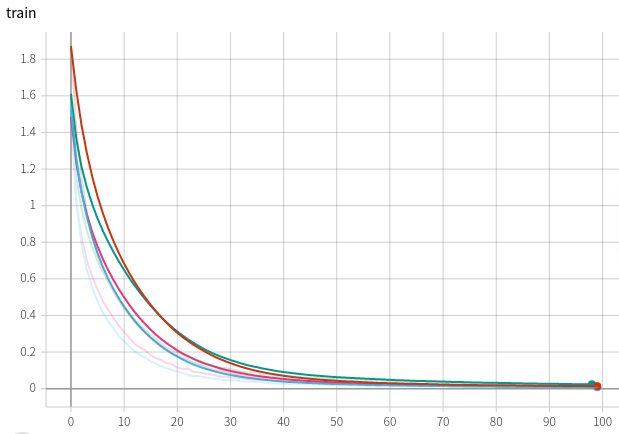
\includegraphics[scale=0.4]{6.png}
\caption{large learning rate}
\end{minipage}
}
\centering
\caption{loss curves with Adadelta}
\end{figure}

\end{itemize}

\section{ResNet}

Since there are several models in ResNets and train a model once needs much time, I just trained ResNet-18 with different hyper parameters and deeper ResNets with same hyper parameter. Hyper parameters and result of each model are shown as following:
 
\begin{itemize}
\item In this part, replace the fc layer for all nets with a new fc layer initialized with \textbf{nn.init.normal\_(params, mean=0.0, std=0.1)}
\item The accuracies of ResNet-18 are shown in table 3. Generally It performs well.
\begin{itemize}
\item As learning rate becomes smaller, net performs better since loss can be more closer to minimum point.
\item Since larger batch size will run out of memory, small batch size is more used here. Within this scale, larger batch size works better.
\end{itemize}

\begin{table}[h]
\caption{momentum=0.9, epochs=10}
%\label{sample-table}
\begin{center}
\begin{tabular}{c|c|c}
\multicolumn{1}{c}{\bf Learning Rate} & \multicolumn{1}{c}{\bf Batch Size} &\multicolumn{1}{c}{\bf Accuracy}
\\ \hline \\
0.01 & 8 & 86.18\% \\
0.01 & 16 & 91.59\% \\
0.01 & 32 & 92.99\% \\
0.003 & 8 & 94.93\% \\
0.003 & 16 & 95.68\% \\
0.003 & 32 & 95.53\% \\
0.001 & 8 & 92.15\% \\
0.001 & 16 & 95.56\% \\
\end{tabular}
\end{center}
\end{table}

\item ResNet-34, ResNet-50, ResNet-101 are also trained with the hyper parameters performing best in ResNet-18. The Accuracies are shown in table 4 and their loss curves are shown in Figure 4.

\begin{table}[h]
\caption{learning\_rate0.003, batch\_size=16, momentum=0.9, epochs=20}
%\label{sample-table}
\begin{center}
\begin{tabular}{c|c}
\multicolumn{1}{c}{\bf Net} &\multicolumn{1}{c}{\bf Accuracy}
\\ \hline \\
ResNet-18 & 95.68\% \\
ResNet-34 & 95.32\% \\
ResNet-50 & 95.45\% \\
ResNet-101 & 96.23\% \\
\end{tabular}
\end{center}
\end{table}

\begin{figure}[ht]
	\centering
	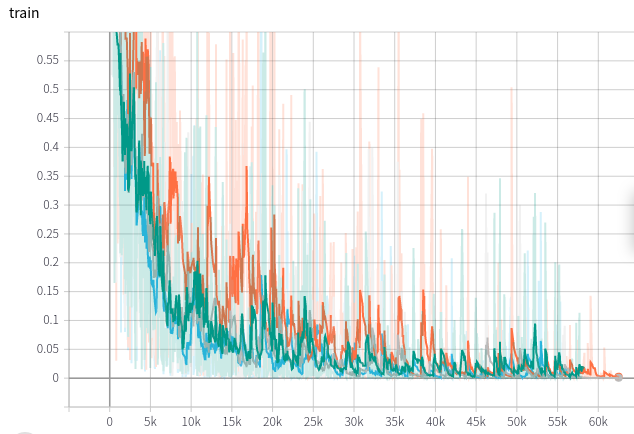
\includegraphics[width=0.4\textwidth]{5.png}
	\caption{ResNets Loss Curves}
	\label{fig:f2}
\end{figure}

\end{itemize}

\section{Summary of Mini Project}
Generally Mini project has come to an end. The best performances of these three models are shown as following:

\begin{itemize}
\item AlexNet: with learning rate=0.01, batch size=128, momentum=0.9, get accuracy of 88.09\%.

\item VGG Net: with learning rate=0.0003, batch size=8, momentum=0.9, get accuracy of 91.10\%.

\item ResNets: ResNet-101 with learning rate=0.003, batch size=16, momentum=0.9, get accuracy of 96.23\%.


\begin{figure}[htbp]
\centering
{
\begin{minipage}[t]{0.45\textwidth}
\centering
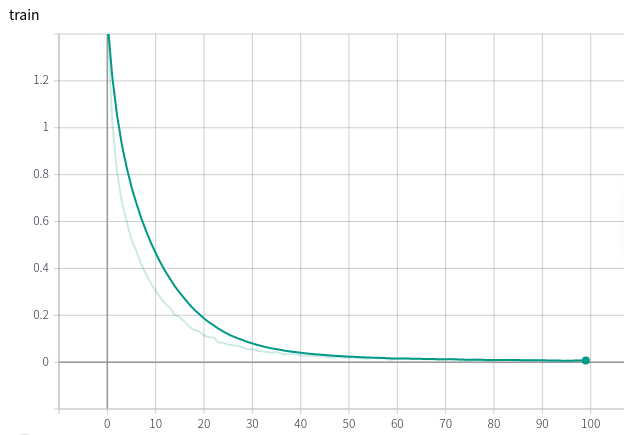
\includegraphics[scale=0.3]{3.png}
\caption{AlexNet Loss Curve}
\end{minipage}
}
{
\begin{minipage}[t]{0.45\linewidth}
\centering
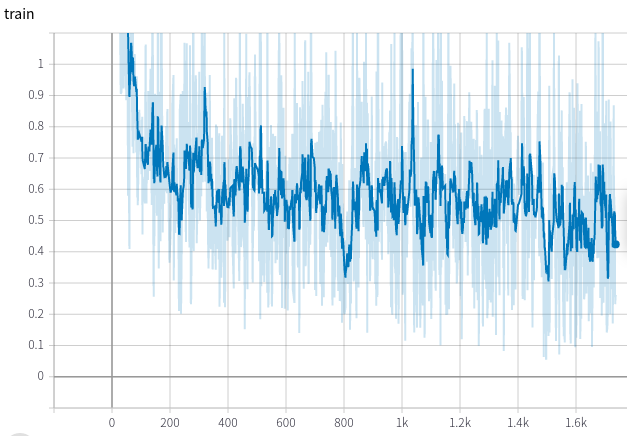
\includegraphics[scale=0.3]{4.png}
\caption{VGG Loss Curve}
\end{minipage}
}
{
\begin{minipage}[t]{0.45\linewidth}
\centering
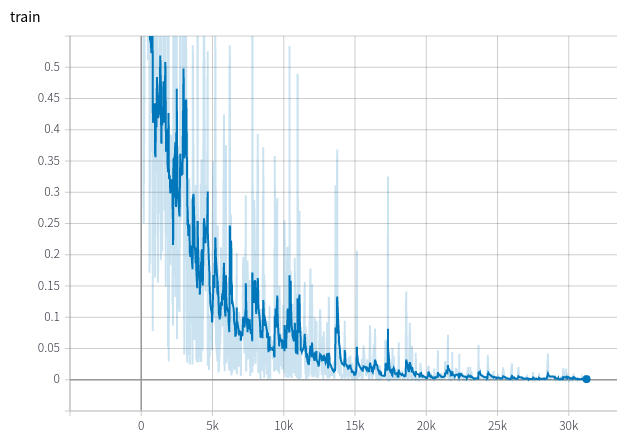
\includegraphics[scale=0.3]{2.png}
\caption{ResNet Loss Curve}
\end{minipage}
}
\centering
\caption{loss curves of best performance}
\end{figure}

\end{itemize}

\end{document}
